\chapter{常微分方程数值解}
\begin{introduction}
\item 定义与分类
\item 数值解方法
\item MATLAB中微分方程的表示方法
\item ode45函数
\end{introduction}
\section{常微分方程}
\subsection{定义}
含有未知函数导数的方程。
\subsection{分类}
分为\textbf{初值问题}与\textbf{边值问题}。

本节主要关注利用\textbf{步进法}解决\textbf{初值问题}。
\subsection{初值问题的数值解方法}
\begin{itemize}
	\item 欧拉法:单步,矩形公式;
	\item 龙格-库塔法:单步,线性组合;
	\item 阿达姆斯法:多步。
\end{itemize}
\section{MATLAB解常微分方程}
\subsection{微分方程的表示}
对于\textcolor{third}{\textbf{微分方程}}:
\[y'=2x+y\]
\begin{lstlisting}[frame=single,numbers=left]
% 可表示为
function dy=odefun(x,y)
dy=2*x+y

% 或
odefun=@(x,y) 2*x+y
\end{lstlisting}

对于\textcolor{third}{\textbf{微分方程组}}:
\[
\begin{cases}
y_1'=y_1-y_2+x\\
y_2'=y_1'+y_2
\end{cases} \]

\begin{lstlisting}[frame=single,numbers=left]
% 可表示为
function dy=odefun(x,y)
dy1=y(1)-y(2)+x;
dy2=dy1+y(2);
dy=[dy1;dy2]; %方程组的dy用列向量输出!
\end{lstlisting}

对于\textcolor{third}{\textbf{高阶微分方程组}}:
\[
\begin{cases}
y_1'=xy_2'+y_1\\
y_2''=y_1'+sin(x)y_2
\end{cases} \]

\begin{lstlisting}[frame=single,numbers=left]
% 变量代换
% 令y(1)=y1,y(2)=y2,y(3)=y2'
% 可表示为
function dy=odefun(x,y)
dy1=0;dy2=0;ddy2=0;
dy1=x*ddy2+y1;
dy2=y(3);
ddy2=dy1+sin(x)*y(2);
dy=[dy1;dy2;ddy2];
\end{lstlisting}

\subsection{ode45函数}
\begin{lstlisting}[frame=single,numbers=left]
% 常用形式
[T,Y]=ode45(fun,TSPAN,Y0)% TSPAN 求解区间;Y0 初值
% 带参数
[T,Y]=ode45(fun,TSPAN,Y0,options)
% 常用求解参数
%输出T与Y的关系图,类似plot(T,Y)
options=odeset(‘outputfcn’,‘odeplot’) 
%输出求解变量Y之间的二维相平面图,类似plot(Y(2),Y(2))
options=odeset('outputfcn','odephas2') 
\end{lstlisting}

\newpage
\begin{problem}
某串联反应各物质的浓度与反应时间 $t$ 的关系如下\footnote{改自隋志军老师“课程练习题”}:
\[
	\begin{cases}
		\frac{\dd{C_{A}}}{\dd{t}} = - k_{1} C_{A} \\
		\frac{\dd{C_{B}}}{\dd{t}} = k_{1} C_{A} - k_{2} C_{B} \\
		\frac{\dd{C_{C}}}{\dd{t}} = k_{2} C_{B} - k_{2} C_{C} \\
		\frac{\dd{C_{D}}}{\dd{t}} = k_{3} C_{C} - k_{4} C_{D} \\
		\frac{\dd{C_{E}}}{\dd{t}} = k_{4} C_{D}
	\end{cases}
\]
\begin{figure}[htbp]
\centering
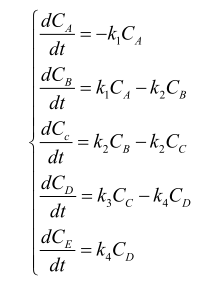
\includegraphics[width=0.4\textwidth]{ode.png}
\end{figure}
\\已知 $k_{1} = 0.04$,$k_{2}=0.05$,$k_{3}=0.10$,$k_{4}=0.08$,反应开始时只有 A 存在,其浓度为 1。
试编写一个 MATLAB 函数,求前 \SI{60}{s} 中每隔 \SI{5}{s} 时各物质的浓度,并作图。
\end{problem}

\begin{solution}

\begin{lstlisting}
function solveC
T=0:5:60;
C0=[1 0 0 0 0];
% 设置图形输出
options=odeset('outputfcn','odeplot');
% 核心函数
[T C]=ode45(@odefun,T,C0,options);
% 常微分方程组
function dC=odefun(T,C)
k1=0.04;k2=0.05;k3=0.10;k4=0.08;
dCA=-k1*C(1);
dCB=k1*C(1)-k2*C(2);
dCC=k2*C(2)-k2*C(3);
dCD=k3*C(3)-k4*C(4);
dCE=k4*C(4);
dC=[dCA;dCB;dCC;dCD;dCE]; %按列
\end{lstlisting}

\end{solution}




